Durch die gestiegene Rechenleistung der heutigen Computer ist auch die Anwendungshäufigkeit von Genetischen Algorithmen deutlich gestiegen. Es werden nicht nur neue Ansätze und Grundlagen erforscht, sondern auch erste Anwendungen entwickelt. Diese finden nicht nur im IT-Bereich, sondern auch in den Naturwissenschaften Anwendung. Der erste Abschnitt befasst sich mit aktuellen Forschungsschwerpunkten im Bereich der Genetischen Algorithmen. Im zweiten Abschnitt wird auf die Anwendungen zu Genetischen Algorithmen eingegangen.

\section{Stand der Forschung}

\subsection{Deep Mind}
Den größten Fortschritt im Bereich der Optimierung von Hyperparametern  verzeichnete Googles Deepmind. Deepmind setzt dabei auf einen populationsbasierenden Algorithmus, welcher den Genetischen Algorithmen ähnelt. Das PopulationBasedTraining \cite{pbt}, wird vor allem im Bereich der künstlichen Intelligenz für Brett- und Computerspiele erforscht. So konnte Deepmind bei verschiedenen künstlichen neuronalen Netzen wie AlphaGo(Go) \cite{alphago} und AlphaStar(Starcraft2) \cite{alphastar} deutliche Verbesserungen erreichen. Das PBT wird aber nicht nur für Spiele genutzt, sondern auch für Anwendungen im Bereich des autonomen Fahrens. Dort wurde in Zusammenarbeit mit der Google-Tochter Waymo eine Verbesserung der Zuverlässigkeit ihrer künstlichen neuronalen Netze ausgearbeitet. Sie konnten eine Reduzierung um 24\% der falsch positiven Klassifikationsergebnisse gegenüber den von hand-modifizierten Netzen erreichen und dies bei gleichbleibender Recallrate. Mithilfe der neu berechneten Hyperparameter, wurden die alten KNN von Waymo deutlich übertroffen und das bei der Hälfte an Trainingszeit und Ressourcen. Somit hat Google Deepmind in mehreren Fällen gezeigt, dass ihre PBT eine deutliche Verbesserung in der Optimierung von Hyperparametern ist. \cite{Waymo}


\subsection{PopulationBasedTraining}
Populationsbasiertes Training (PBT) ist eine Kombination aus Random-Search (Siehe Kap.\ref{Zufalls_Suche}) und Genetischen Algorithmen (Siehe Kap.\ref{Genetische_Algorithmen}). Der zu Grunde liegende Suchalgorithmus ist ein heuristischer Suchansatz mit einer Kandidatenlösungsmenge. Des Weiteren wurden Methoden wie "`Survival of the Fittest"' und Mutation aus dem Genetischen Algorithmus übernommen. Darüber hinaus wurde ein online Anpassung der Hyperparameter während des Trainings implementiert. Schlechte Worker (Worker sind gleichzusetzen mit Individuen von GA) werden durch Worker mit besserem Fitnesswert ersetzt(exploit). Sie werden nicht einfach ersetzt, sondern erhalten kleine Mutationen(explore). Diese Worker müssen nicht von Beginn neu trainiert werden, sondern können auf die Gewichtungen der Eltern zurückgreifen. Dies ist gut in Abbildung \ref{fig:pbt} zusehen. Die Online-Anpassung ist dabei die größte Verbesserung. Es kann mit einem Pool beim Multiprocessing verglichen werden. Nach Beenden der Berechnung der Fitness wird direkt mit der Fitness eines neues Workers begonnen, ohne dass dabei auf andere Worker gewartet werden muss\cite{pbt}. 

\noindent%
\begin{figure}[h]
  \centering  
  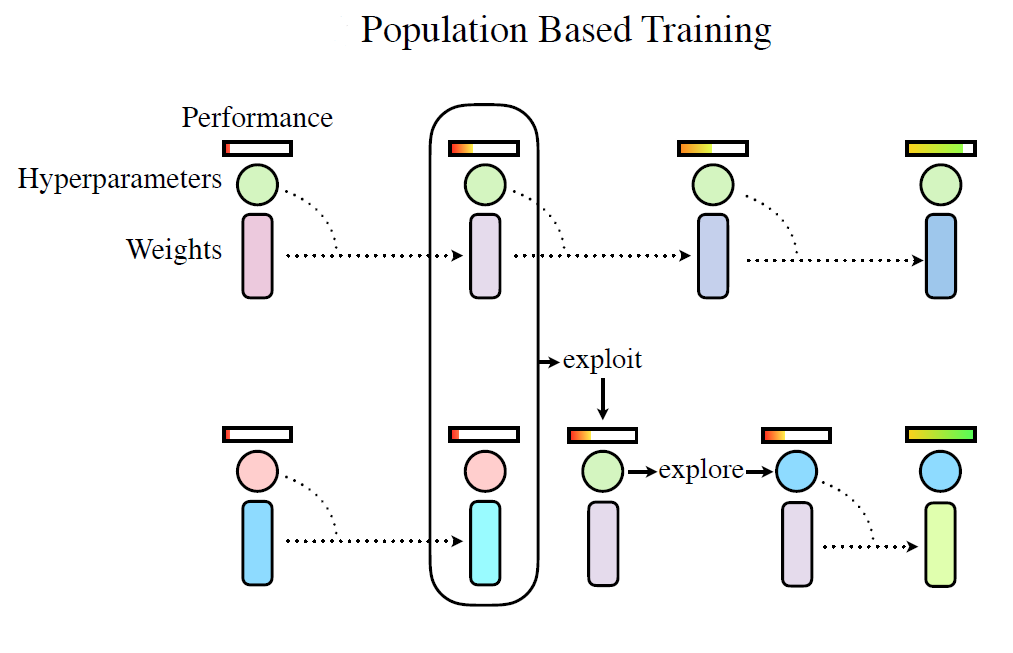
\includegraphics[scale=0.3]{img/pbt.png}
  \caption{Population Based Training \cite{pbt}}
  \label{fig:pbt}
\end{figure}

\subsection{NeuroEvolution of Augmenting Topologies(NEAT)}
NEAT ist ein Optimierungsverfahren für Modell-Architekturen von KNNs. Dabei wird die Topologie der Netze und Gewichte verbessert. Die Entwickler von NEAT konnten mit ihrem Algorithmus zeigen, dass es möglich ist, Netze zu optimieren und gleichzeitig komplexer zu gestalten. Der Algorithmus baut auf den Genetischen Algorithmen auf. Das Netz wird so einfach wie möglich initialisiert, somit wird mit schlechter Performance gestartet und über Generationen wird das Netz komplexer. Es wird mit mehr Neuronen und Verbindungen versehen und somit qualitativ verbessert. In Abbildung \ref{fig:gene-neat} ist ein Chromsomenstrang zu sehen mit den Verbindungs-Genen (engl. Connection Genes) aus welchen die Neuronen-Gene (engl. Node Genes) erstellt werden können. Über die Mutation können einzelne Verbindungen(Gewichte) hinzugefügt werden, zu sehen in Abbildung \ref{fig:crossover-neat}.

\noindent%
\begin{figure}[h]
  \centering  
  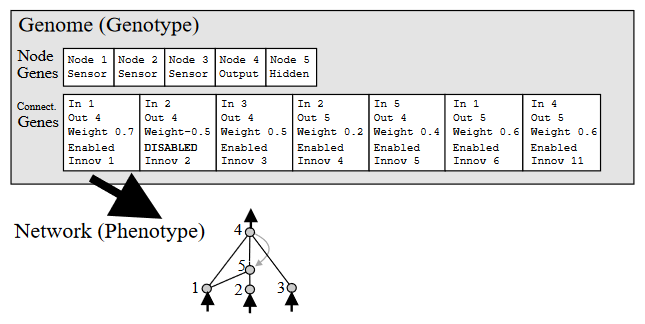
\includegraphics[scale=0.7]{img/gene-neat.png}
  \caption{Aufbau eines Chromosomes bei NEAT \cite{stanley2002evolving}}
  \label{fig:gene-neat}
\end{figure}

Somit wird das Netz komplexer. Durch Hinzufügen von Gewichten (weights) wächst die Länge des Chomosomstrangs. Es werden zufällig auch einzelne Verbindungen ausgeschaltet, um ihre Nützlichkeit zu überprüfen. Sie können zu späteren Zeitpunkten zufällig wieder aktiviert werden. Dies ist in Abbildung \ref{fig:crossover-neat} im Chromenstrang zusehen und als "`DISAB"' markiert. Für die Eltern-Auswahl werden die Netze mit ähnlicher Struktur in sogenannte Spezies eingeteilt. Nun wird von jeder Spezies die schlechtere Hälfte an Individuen gelöscht. Damit ist die Eltern-Selektion nicht direkt von der Fitness abhängig und gibt schlechteren Individuen eine Überlebenschance und somit auch die Möglichkeit, sich weiter zu entwickeln. Crossover funktioniert bei NEAT ähnlich wie beim klassischen Genetischen Algorithmus. Der Unterschied liegt darin, dass die Gene addiert werden. Dies bedeutet, Verbindungen, die nur in einem Individuum vorkommen, werden an die Nachkommen übergeben. Wenn ein Gen ausgeschaltet ist, wird es im Nachkommen mit hoher Wahrscheinlichkeit auch ausgeschaltet sein. Da nun die Nachkommen gebildet wurden, kann aus diesen eine neue Generation gebildet werden und der Optimierungsprozess beginnt von Neuem. Diese Optimierung ist nicht Teil der Arbeit und dient nur zur Information für vergleichbaren Forschungsarbeiten.\cite{stanley2002evolving}

\noindent%
\begin{figure}[h]
  \centering  
  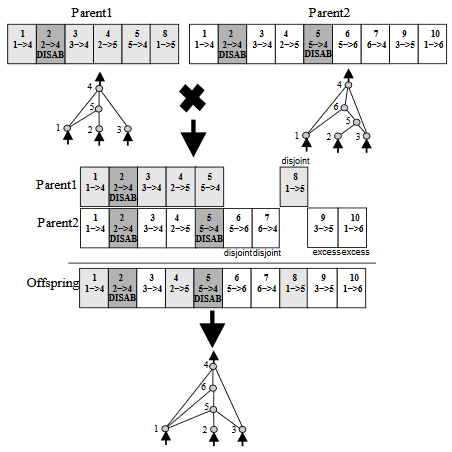
\includegraphics[scale=0.9]{img/crossover-neat.png}
  \caption{Crossover bei Neat \cite{stanley2002evolving}}
  \label{fig:crossover-neat}
\end{figure}

\newpage

\section{Stand der Technik}
\subsection{Software Testing mit GA}
Die Softwarebewertung spielt eine entscheidende Rolle im Lebenszyklus eines Software-Produktionssystems. Die Erzeugung geeigneter Daten zum Testen des Verhaltens der Software ist Gegenstand vieler Forschungen im Software-Engineering. So wurde von Keshavarz und Kollegen die Qualitätskontrolle mit Kriterien zur Abdeckung von Anwendungspfaden betrachtet und hierfür ein neues Verfahren auf der Grundlage eines genetischen Algorithmus zur Erzeugung optimaler Testdaten entwickelt\cite{Keshavarz}. 


\subsection{Temperatur Schätzungen}
Genetische Algorithmen werden auch zur Berechnung von Temperaturverläufen eingesetzt \cite{Stanislawska1}. Als Eingangsdaten werden verschiedene Daten benutzt, wie beispielsweise: Sonnenaktivität, Vulkanausbrüche und Greenhouse-Gasanteil in der Atmosphäre. Als Ausgabe erhalten wir dann eine Abschätzung der Temperatur für die nächsten Jahre. Von den gleichen Autoren gibt es auch eine Berechnung der Abschätzungen des Wärmeflusses zwischen Atmosphäre und Meereis in Polarregionen \cite{Stanislawska2}. All diese Vorhersagen wurden mithilfe von der Genetischen Programmierung berechnet. Als Trainingstag wurden Aufzeichnungen von Temperaturverläufen und anderen Eingangsdaten der letzten Jahrhunderte verwendet.

\subsection{Generatives Design}
In den letzten Jahren ist die Komplexität von CAD Programmen (engl. Computer-Aided Design) deutlich gestiegen. Diese enthalten nun auch Implementierungen von Generativen Design-Werkzeugen. Mithilfe dieser Generativen Design-Werkzeugen ist es möglich, aus klassischen Bauteilen bionische Bauteile zu entwicklen. Hierfür werden die Bauteile über Iterationen optimiert. So kann aus einem Bauteil, ein wesentlich leichteres und materialsparenderes Modell entwickelt werden. In Abbildung \ref{fig:additives} sind verschiedene Schritte des Generativen Designs zu sehen. Die Fertigung ist meist nur mit additiven Fertigungsmethoden möglich, da die berechneten Strukturen keinen Fertigungsregeln unterliegen\cite{caldas2008generation}. 

\begin{figure}[h]
  \centering  
  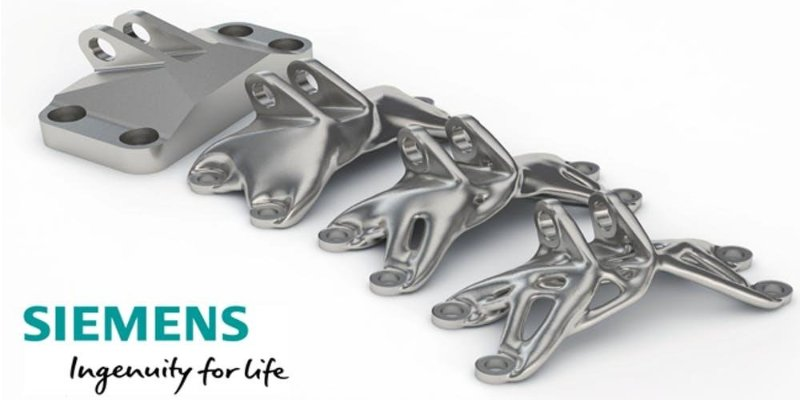
\includegraphics[scale=0.4]{img/Additive.png}
  \caption{Additives Design Beispiel von Siemens \cite{siemens}}
  \label{fig:additives}
\end{figure}

\paragraph{NASA - Antenne}
Dieser Generative Algorithmus wurde schon 2006 von der NASA erforscht. Hierbei wurde eine Weltraumantenne mit Hilfe von evolutionären Algorithmen entwickelt. In Abbildung \ref{fig:nasa} sind zwei Prototypen der Weltraumantenne zu sehen. Die Entwicklung einer solchen Antenne braucht enormes Wissen in verschiedenen Domänen wodurch die Entwicklung sehr arbeitsintensiv und somit auch Zeitaufwändig wäre. Deshalb benutzen die Forscher einen populationsbezogenen Suchansatz, um Umgebungsstrukturen und elektromagnetische Auswirkungen mit einzubeziehen. Die entwickelte Antenne wurde produziert und auch auf der Space Technology 5 Mission genutzt \cite{AutomatedAntenna}.

\begin{figure}[h]
  \centering  
  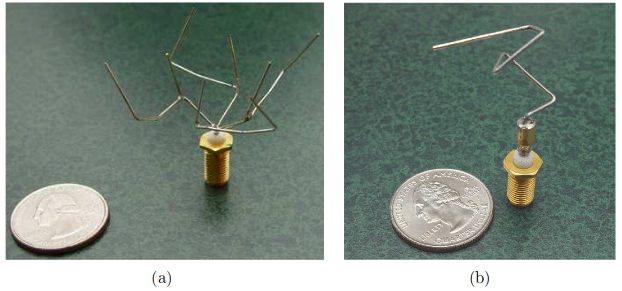
\includegraphics[scale=0.5]{img/nasa-antenne.png}
  \caption{Foto der Prototypen \cite{AutomatedAntenna}}
  \label{fig:nasa}
\end{figure}

\newpage

\section{Zusammenfassung}
In diesem Kapitel wurde der Stand der Technik und Forschung für Optimierung und Genetische Algorithmen erläutert. Dazu wurde erst das Populations Basiertes Training(PBT) von Google Deepmind erläutert, welches auf den Genetischen Algorithmen basiert und zur Optimierung von Hyperparametern bei künstlichen neuronalen Netzen angewendet wird. Des Weiteren wurde NeuroEvolution of Augmenting Topologies(NEAT) vorgestellt, dies wird auch zur Optimierung von KNN verwendet. NEAT basiert auch auf dem Genetischen Algorithmus, verwendet aber einen anderen Ansatz wie das PBT oder der klassische GA. Bei NEAT wird die Modell-Architektur optimiert. Dazu wird mit dem kleinstmöglichen Netz angefangen und anschließend über viele Iterationen Verbindungen und Neuronen hinzugefügt, so dass sich die Qualität des Netzes verbessert. Abschließend wurden einige Beispiele aufgezählt, in welchen GA angewendet werden. Diese sind: Temperaturabschätzung, Software Testing und Generatives Design.